%!TEX root = ../main.tex 

\section{Pourquoi une impédance?}

\begin{frame}{Différence de phase entre réactances}
    \begin{figure}
        \centering
        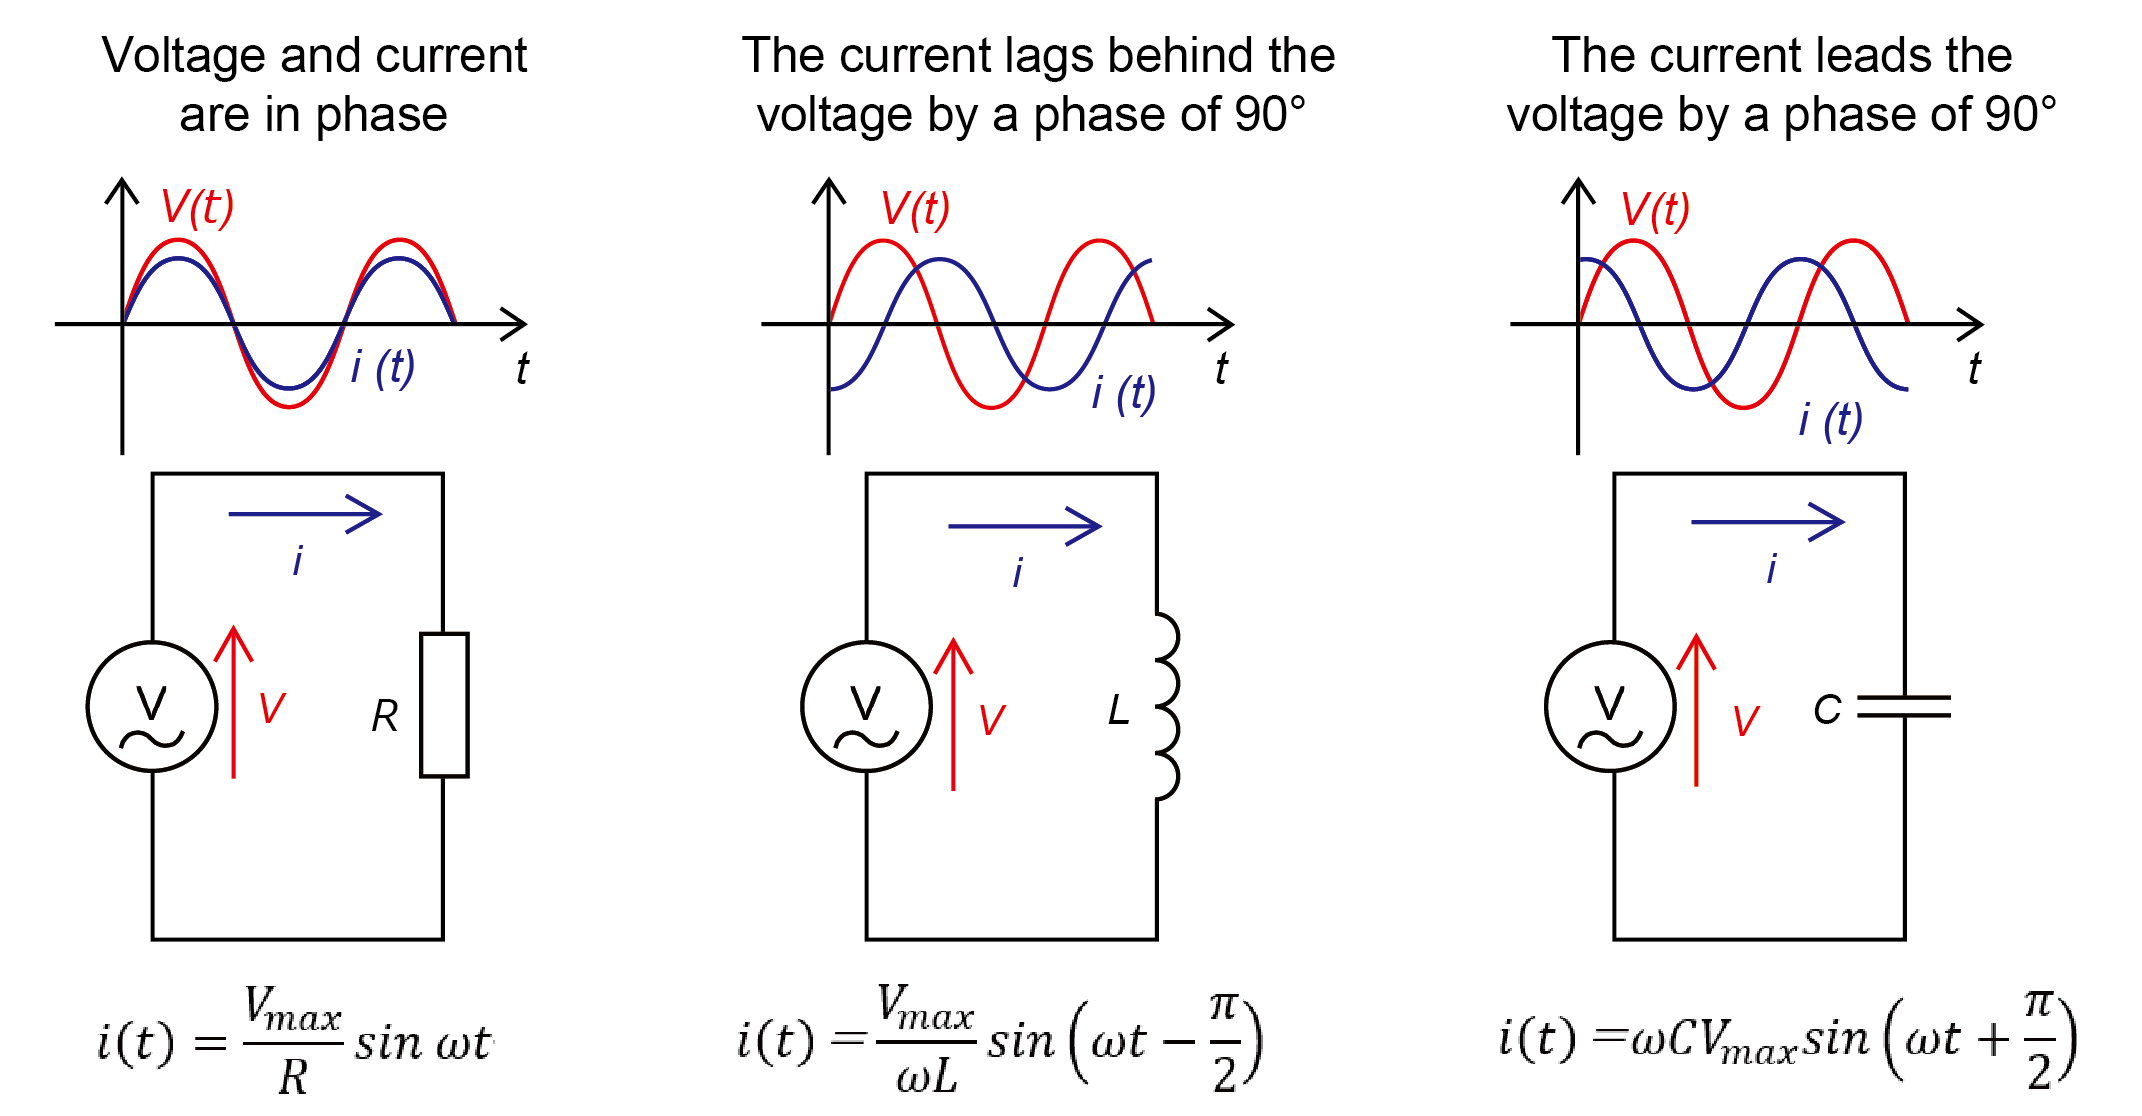
\includegraphics[width=\textwidth]{pictures/Phase_Difference_Between_Impedance_and_Current.png}
    \end{figure}
\end{frame}

\begin{frame}{Power Factor}
    \begin{columns}
        \begin{column}{0.5\textwidth}
            \begin{itemize}
                \item Ratio du \textit{vrai} power ($kW$) au power \textit{apparent} ($kVA$).
                \item Avec impédance imaginaire vient puissance imaginaire
                \item Seule la puissance réelle est utile
            \end{itemize}
            \begin{figure}
                \centering
                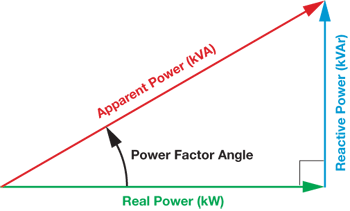
\includegraphics[width=\textwidth]{pictures/power-factor.png}
            \end{figure}
        \end{column}
        \begin{column}{0.5\textwidth}
            \begin{figure}
                \centering
                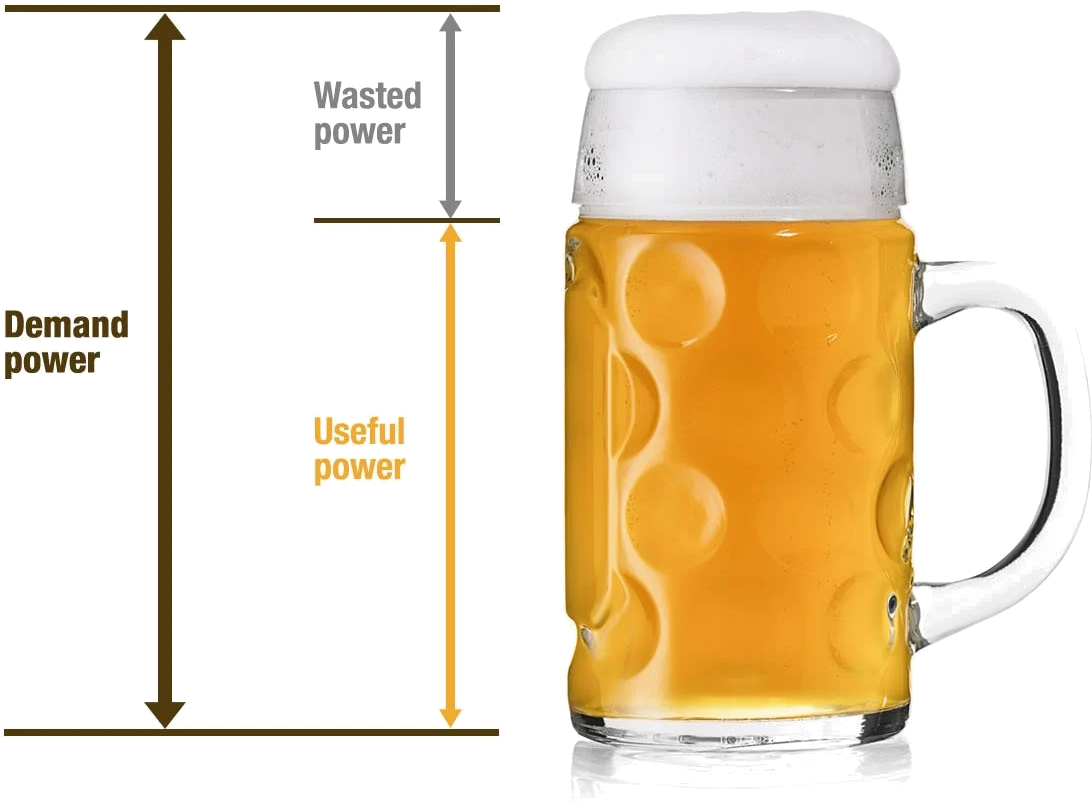
\includegraphics[width=\textwidth]{pictures/power-factor-beer.png}
            \end{figure}
        \end{column}
    \end{columns}
\end{frame}


\subsection{Réflexions}

\begin{frame}{Ligne de transmission - Circuit Ouvert}
    \begin{center}

    \Large{$i = \frac{V}{Z_0}$}
    
    \resizebox{0.9\textwidth}{!}{
    \begin{circuitikz}[american voltages]
        \draw [thick]
        (0,0) to [short, *-*] (8,0)
        to [open, -*] (8,4)
        (0,0) to [open, v<=$5V$] (0,4)
        to [short, *- ,i=$i$, a=$100mA$] (4,4)
        to [european resistor, l=$Z_0$, a=$50\Omega$] (6, 4)
        to [short, -*] (8,4)
        ;
        \draw[thick, dashed]
        (8, 4) to [short] (8, 3)
        to [short, a=\mbox{$i_L=0A$}] (8, 2)
        to [short, a=\mbox{$Z_L = \infty$}] (8, 1)
        to [short] (8, 0);
    \end{circuitikz}
    }
    \end{center}
\end{frame}

\begin{frame}{Circuit Ouvert - Onde à envoyer}
    \begin{center}
        \begin{tikzpicture}
            \begin{axis}[
                axis lines = left,
                xlabel = \(t\),
                ylabel = \(V\),
                ymax = 3.3,
                xmax = 10,
            ]
            \addplot [
                domain=0:10,
                thick,
                color=red,
            ]
            coordinates
            {(0, 0) (1, 0) (1.5, 1) (6, 1) (6.5, 0) (10, 0)};
            \addlegendentry{\(Input\ Voltage\)}
            \end{axis}
        \end{tikzpicture}
    \end{center}
\end{frame}

\begin{frame}{Circuit Ouvert}
    \begin{center}
        \begin{tikzpicture}
            \begin{axis}[
                axis lines = left,
                xlabel = \(p\),
                ylabel = \(V\),
                ymax = 3.3,
                xmax = 10,
                title={t = 2},
            ]
            \addplot [
                domain=0:10,
                thick,
                color=red,
            ]
            coordinates
            {(0, 1) (1, 1) (1.25, 0) (10, 0)};
            \end{axis}
        \end{tikzpicture}
    \end{center}
\end{frame}

\begin{frame}{Circuit Ouvert}
    \begin{center}
        \begin{tikzpicture}
            \begin{axis}[
                axis lines = left,
                xlabel = \(p\),
                ylabel = \(V\),
                ymax = 3.3,
                xmax = 10,
                title={t = 3},
            ]
            \addplot [
                domain=0:10,
                thick,
                color=red,
            ]
            coordinates
            {(0, 1) (7, 1) (7.25, 0) (10, 0)};
            \end{axis}
        \end{tikzpicture}
    \end{center}
\end{frame}

\begin{frame}{Circuit Ouvert}
    \begin{center}
        \begin{tikzpicture}
            \begin{axis}[
                axis lines = left,
                xlabel = \(p\),
                ylabel = \(V\),
                ymin = 0,
                ymax = 3.3,
                xmax = 10,
                title={t = 4},
            ]
            \addplot [
                domain=0:10,
                thick,
                color=red,
            ]
            coordinates
            {(0, 1) (8, 1) (8.25, 2) (10, 2)};
            \end{axis}
        \end{tikzpicture}
    \end{center}
\end{frame}

\begin{frame}{Circuit Ouvert}
    \begin{center}
        \begin{tikzpicture}
            \begin{axis}[
                axis lines = left,
                xlabel = \(p\),
                ylabel = \(V\),
                ymin = 0,
                ymax = 3.3,
                xmax = 10,
                title={t = 7},
            ]
            \addplot [
                domain=0:10,
                thick,
                color=red,
            ]
            coordinates
            {(0, 0) (1, 0) (1.25, 1) (3, 1) (3.25, 2) (10, 2)};
            \end{axis}
        \end{tikzpicture}
    \end{center}
\end{frame}

\begin{frame}{Circuit Ouvert}
    \begin{center}
        \begin{tikzpicture}
            \begin{axis}[
                axis lines = left,
                xlabel = \(p\),
                ylabel = \(V\),
                ymin = 0,
                ymax = 3.3,
                xmax = 10,
                title={t = 8},
            ]
            \addplot [
                domain=0:10,
                thick,
                color=red,
            ]
            coordinates
            {(0, 1) (2, 1) (2.25, 2) (10, 2)};
            \end{axis}
        \end{tikzpicture}
    \end{center}
\end{frame}

\begin{frame}{Circuit Ouvert}
    \begin{center}
        \begin{tikzpicture}
            \begin{axis}[
                axis lines = left,
                xlabel = \(p\),
                ylabel = \(V\),
                ymin = 0,
                ymax = 3.3,
                xmax = 9,
                title={t = 10},
            ]
            \addplot [
                domain=0:10,
                thick,
                color=red,
            ]
            coordinates
            {(0, 1) (8, 1) (8.25, 2) (10, 2)};
            \end{axis}
        \end{tikzpicture}
    \end{center}
\end{frame}

\begin{frame}{Circuit Ouvert}
    \begin{center}
        \begin{tikzpicture}
            \begin{axis}[
                axis lines = left,
                xlabel = \(p\),
                ylabel = \(V\),
                ymin = 0,
                ymax = 3.3,
                xmax = 10,
                title={t = 10},
            ]
            \addplot [
                domain=0:10,
                thick,
                color=red,
            ]
            coordinates
            {(0, 1) (6, 1) (6.25, 0) (10, 0)};
            \end{axis}
        \end{tikzpicture}
    \end{center}
\end{frame}

\begin{frame}{Circuit Ouvert}
    \begin{center}
        \begin{tikzpicture}
            \begin{axis}[
                axis lines = left,
                xlabel = \(p\),
                ylabel = \(V\),
                ymin = 0,
                ymax = 3.3,
                xmax = 10,
                title={t = 11},
            ]
            \addplot [
                domain=0:10,
                thick,
                color=red,
            ]
            coordinates
            {(0, 1) (1, 1) (1.25, 0) (10, 0)};
            \end{axis}
        \end{tikzpicture}
    \end{center}
\end{frame}

